\documentclass{article}
\usepackage[utf8]{inputenc}
\usepackage{amsmath}
\usepackage{amssymb}
\usepackage{graphicx}
\usepackage{subcaption}

\usepackage{bm}


\newcommand{\dx}{\mathrm{dx}}
\newcommand{\dt}{\mathrm{dt}}

\newcommand{\pd}[2]{\dfrac{\partial#1}{\partial#2}}
\newcommand{\complex}[1]{\bm{#1}}
\renewcommand{\vec}[1]{\bm{#1}}
\newcommand{\I}{\complex{i}}
\newcommand{\kx}{\complex{k_x}}
\newcommand{\ky}{\complex{k_y}}
\newcommand{\kxq}{\complex{k_{x,q}}}
\newcommand{\kyp}{\complex{k_{y,p}}}



\begin{document}

\title{Méthode Numériques: Simulation d'écoulement fluide}
\author{Aurélien Moisson-Franckhauser et Quentin Boyer}
\maketitle

\section{Resolution de l'equation de transport diffusion}

On discretise l'espace en $N_x$ points et le temps en $N_t$ points. On note alors $\mathrm{dx}=\frac{1}{N_x}$ et $\mathrm{dt}=\frac{1}{N_t}$
L'equation devient:


\begin{equation}
	\begin{aligned}
	\phi(x,t+\dt) ={} & \phi(x,t)-c(x)\frac{\dt}{2\dx}(\phi(x+\dx, t)-\phi(x-\dx,t)) \\
					&+c{(x)}^2\frac{\dt^{2}}{2\dx^{2}}(\phi(x+\dx,t)-2\phi(x, t)+\phi{x-\dx}{t}) \\
					&+\kappa\frac{\dt}{\dx^2}(\phi(x+\dx,t+\dt)-2\phi(x,t+\dt)+\phi(x-\dx,t+\dt))
	\end{aligned}
	\label{eq:diff}
\end{equation}


\paragraph{Question 1}
On note pour $0 \leq k \le N_t$:

\[U^{[k]}=
\begin{bmatrix}
	\phi(0, k\dt) \\
	\vdots \\
	\phi(n\dx, k\dt) \\
	\vdots \\
	\phi((N_x-1)\dx, k\dt)
\end{bmatrix}
\]
On note $U_n^{[k]}$ la composante $n$ de $U^{[k]}$. On cherche alors $ M,N \in \mathcal{M}_{N_x}(\mathbb{R})$ telles que $NU^{[k+1]}=MU^{[k]}$.
En utilisant les notations introduites~(\ref{eq:diff}) se reecrit pour $x=n\dx$ et $t=k\dt$:

\[
	\begin{aligned}
		U^{[k+1]}_n ={} & U_n^{[k]} - c(n\dx)\frac{\dt}{2\dx}(U_{n+1}^{[k]}-U_{n-1}^{[k]}) \\
		& +c{(n\dx)}^2\frac{\dt^{2}}{2\dx^{2}}(U_{n+1}^{[k]}-2U_{n}^{[k]}+U_{n-1}^{[k]}) \\
						& +\kappa\frac{\dt}{\dx^2}(U_{n+1}^{[k+1]}-2U_{n}^{[k+1]}+U_{n-1}^{[k+1]})
	\end{aligned}
\]

Soit

\[
	\begin{aligned}
		&-\kappa\frac{\dt}{\dx^2}U_{n-1}^{[k+1]}+(1+2\kappa\frac{\dt}{\dx^2})U_{n}^{[k+1]}-\kappa\frac{\dt}{\dx^2}U_{n+1}^{[k+1]} \\
		&=c(n\dx)\frac{\dt}{2\dx}(c(n\dx)\frac{\dt}{\dx}+1)U_{n-1}^{[k]} + (1-c{(n\dx)}^2\frac{\dt^{2}}{\dx^{2}})U_n^{[k]} + c(n\dx)\frac{\dt}{2\dx}(c(n\dx)\frac{\dt}{\dx}-1)U_{n+1}^{[k]}
	\end{aligned}
\]

On pose $U_{N_x}^{[k]}=U_{0}^{[k]}$ et $U_{-1}^{[k]}=U_{N_x-1}^{[k]}$.

Cela donne donc 

\[
	N =
	\begin{bmatrix}
		(1+2\kappa\frac{\dt}{\dx^2}) & -\kappa\frac{\dt}{\dx^2} & 0 & \hdots & 0 & -\kappa\frac{\dt}{\dx^2} \\
		-\kappa\frac{\dt}{\dx^2} & (1+2\kappa\frac{\dt}{\dx^2}) & -\kappa\frac{\dt}{\dx^2} & 0\\
		0 & \ddots & \ddots &  \ddots & \ddots \\
		\vdots & \ddots & -\kappa\frac{\dt}{\dx^2} & (1+2\kappa\frac{\dt}{\dx^2}) & -\kappa\frac{\dt}{\dx^2} & 0 \\
		0 \\
		-\kappa\frac{\dt}{\dx^2} & 0 & \hdots & 0 & -\kappa\frac{\dt}{\dx^2} & (1+2\kappa\frac{\dt}{\dx^2})
	\end{bmatrix}
\]
$M$ possede une structure similaire mais avec des coefficients differents:
\[
	M =
	\begin{bmatrix}
		(1-c{(0)}^2\frac{\dt^{2}}{\dx^{2}}) & c(0)\frac{\dt}{2\dx}(c(0)\frac{\dt}{\dx}-1) & \hdots & c(0)\frac{\dt}{2\dx}(c(0)\frac{\dt}{\dx}+1)  \\
		c(n\dx)\frac{\dt}{2\dx}(c(n\dx)\frac{\dt}{\dx}+1) & (1-c{(n\dx)}^2\frac{\dt^{2}}{\dx^{2}}) & c(n\dx)\frac{\dt}{2\dx}(c(n\dx)\frac{\dt}{\dx}-1) & 0\\
		0 & \ddots & \ddots &  \ddots & \ddots \\
	\end{bmatrix}
\]

\paragraph{Question 2}
\subparagraph{Matrice $N$ du systeme}

On voit bien que $N^T=N$ donc $N$ est symetrique.
De plus $N$ est une matrice circulante, et posant $a=1+2\kappa\frac{\dt}{\dx^2}$ et $b=-\kappa\frac{\dt}{\dx^2}$ on a le polynome associe a $N$ qui est $f(x)=a+b\left(x+x^{(N_x-1)}\right)$.

Les valeurs propres de $N$ sont alors pour $k=0,\dots,n-1$ $\lambda_k=f\left(\exp\left(i\frac{2\pi k}{N_x}\right)\right)$.
Soit $\lambda_k=a+b\left(\exp\left(i\frac{2\pi k}{N_x}\right)+\exp\left(i\frac{2\pi k(N_x-1)}{N_x}\right)\right)$.

Or $\exp\left(i\frac{2\pi k(N_x-1)}{N_x}\right)=\exp\left(i(-\frac{2\pi k}{N_x}+2\pi k)\right)=\exp\left(-i\frac{2\pi k}{N_x}\right)$

On a donc $\lambda_k=a+b\left(\exp\left(i\frac{2\pi k}{N_x}\right)+\exp\left(-i\frac{2\pi k}{N_x}\right)\right)=a+2b\cos(\frac{2\pi k}{N_x})$

Cela donne $\lambda_k = 1 + 2\kappa\frac{\dt}{\dx^2}\left(1-\cos\left(\frac{2\pi k}{N_x}\right)\right)$

Cette expression est strictement positive puisque $k < N_x$. Donc $\lambda_k > 0$ et $N$ est symetrique definie positive.

\subparagraph{Cholesky} Le fait que la matrice soit symetrique definie positive permet la decomposition de Cholesky. De plus posant $b_k=MU^{[k
-1]}$, on voit qu'on est amenene a resoudre le systeme $NU^{[k]}=b_k$ avec $N$ constante. On resout donc des systemes avec la meme matrice, mais un second membre different. Cela est donc tres adapte a une decomposition de $N$ pour resoudre le systeme.

\paragraph{Question 4}

\begin{figure}
	\centering
	\begin{subfigure}[b]{0.3\textwidth}
		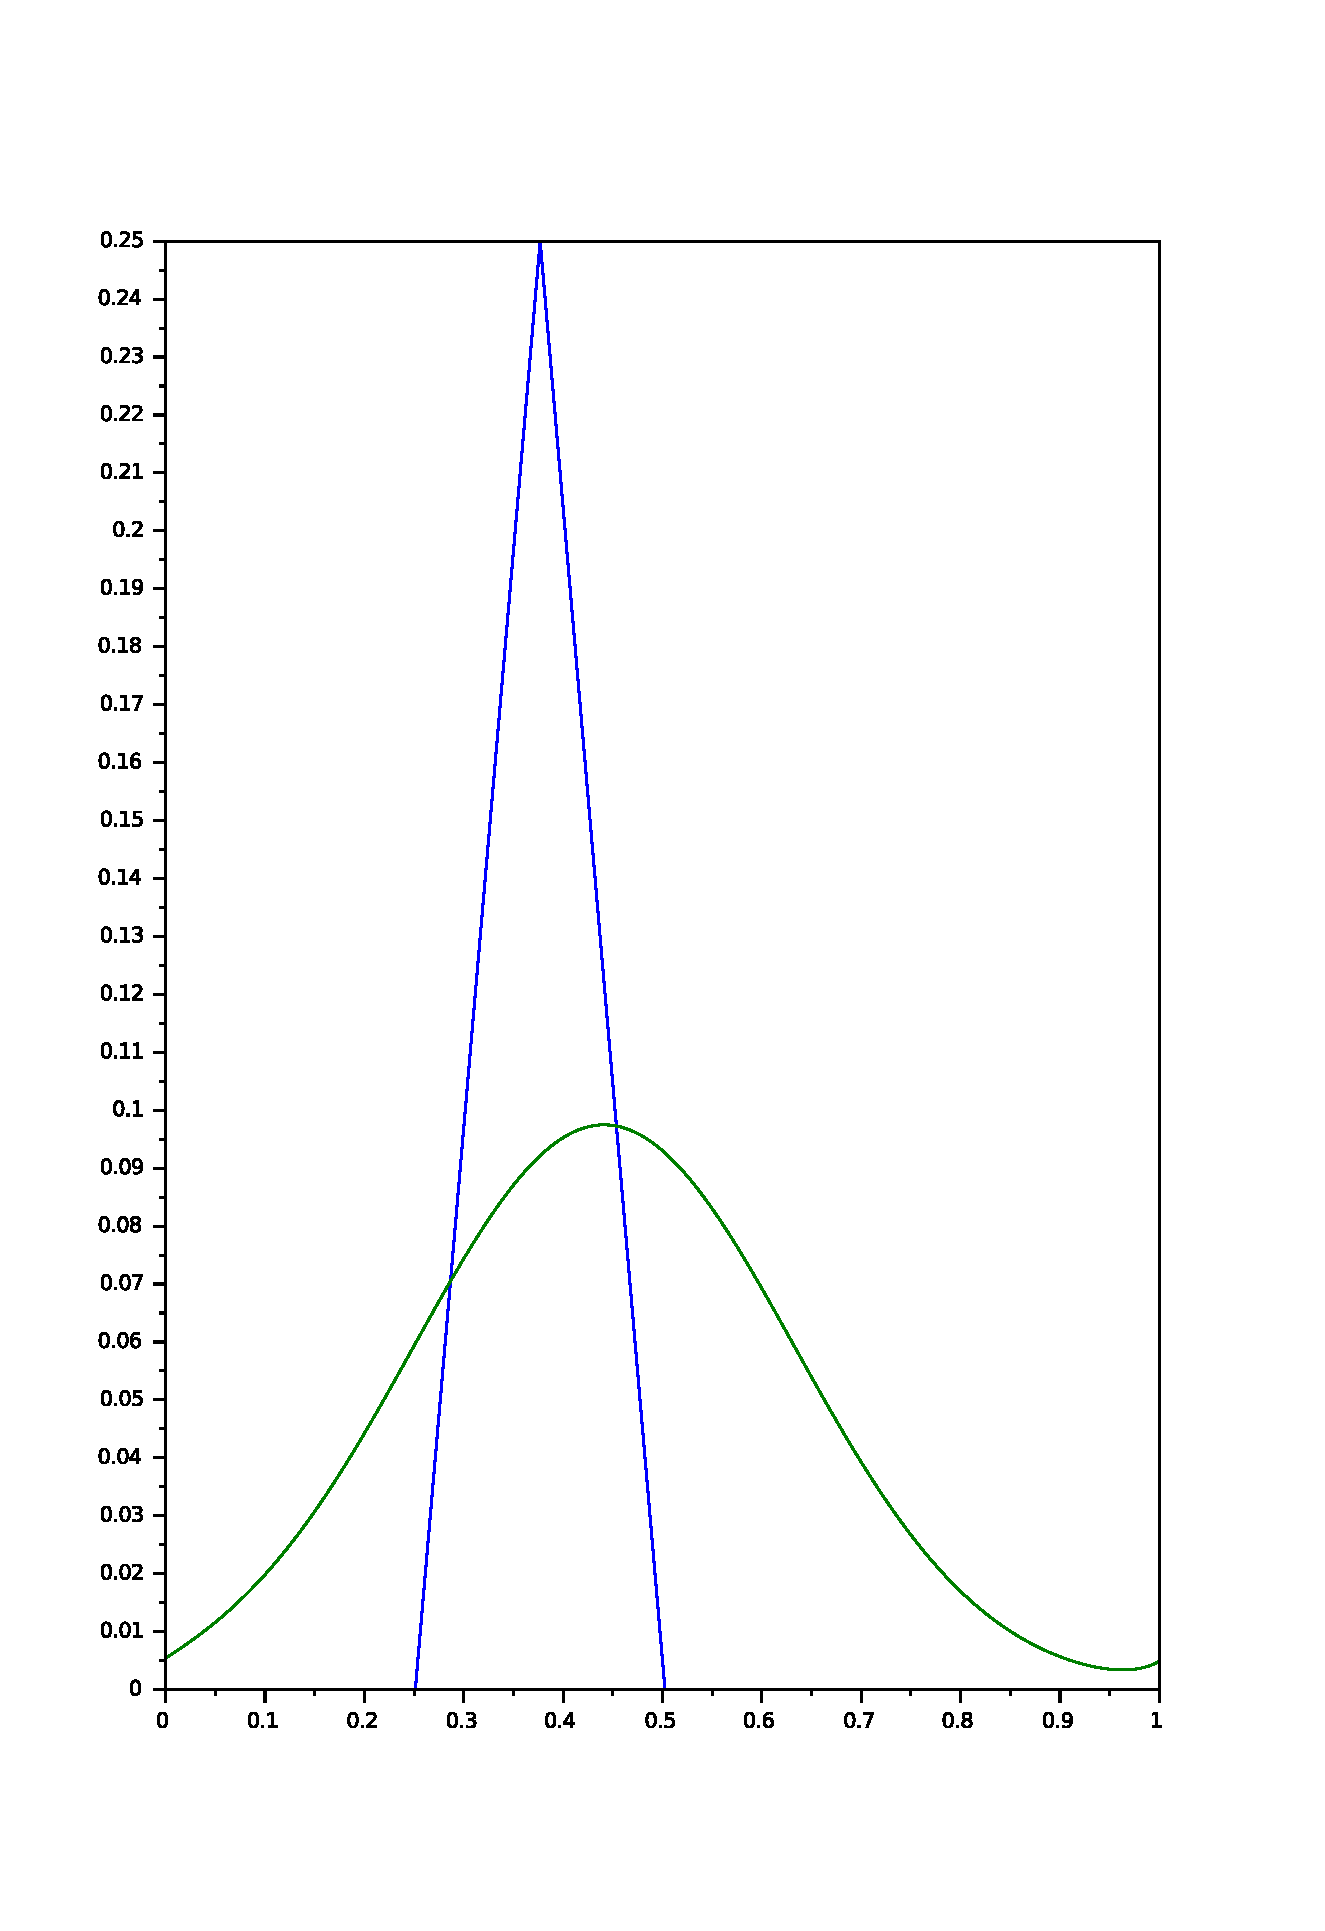
\includegraphics[width=\textwidth]{conv_kappa_0,01.pdf}
		\caption{$\kappa=0.01$}
	\end{subfigure}
	\quad
	\begin{subfigure}[b]{0.3\textwidth}
		\includegraphics[width=\textwidth]{conv_kappa_0,001.pdf}
		\caption{$\kappa=0.001$}
	\end{subfigure}
	\quad
	\begin{subfigure}[b]{0.3\textwidth}
		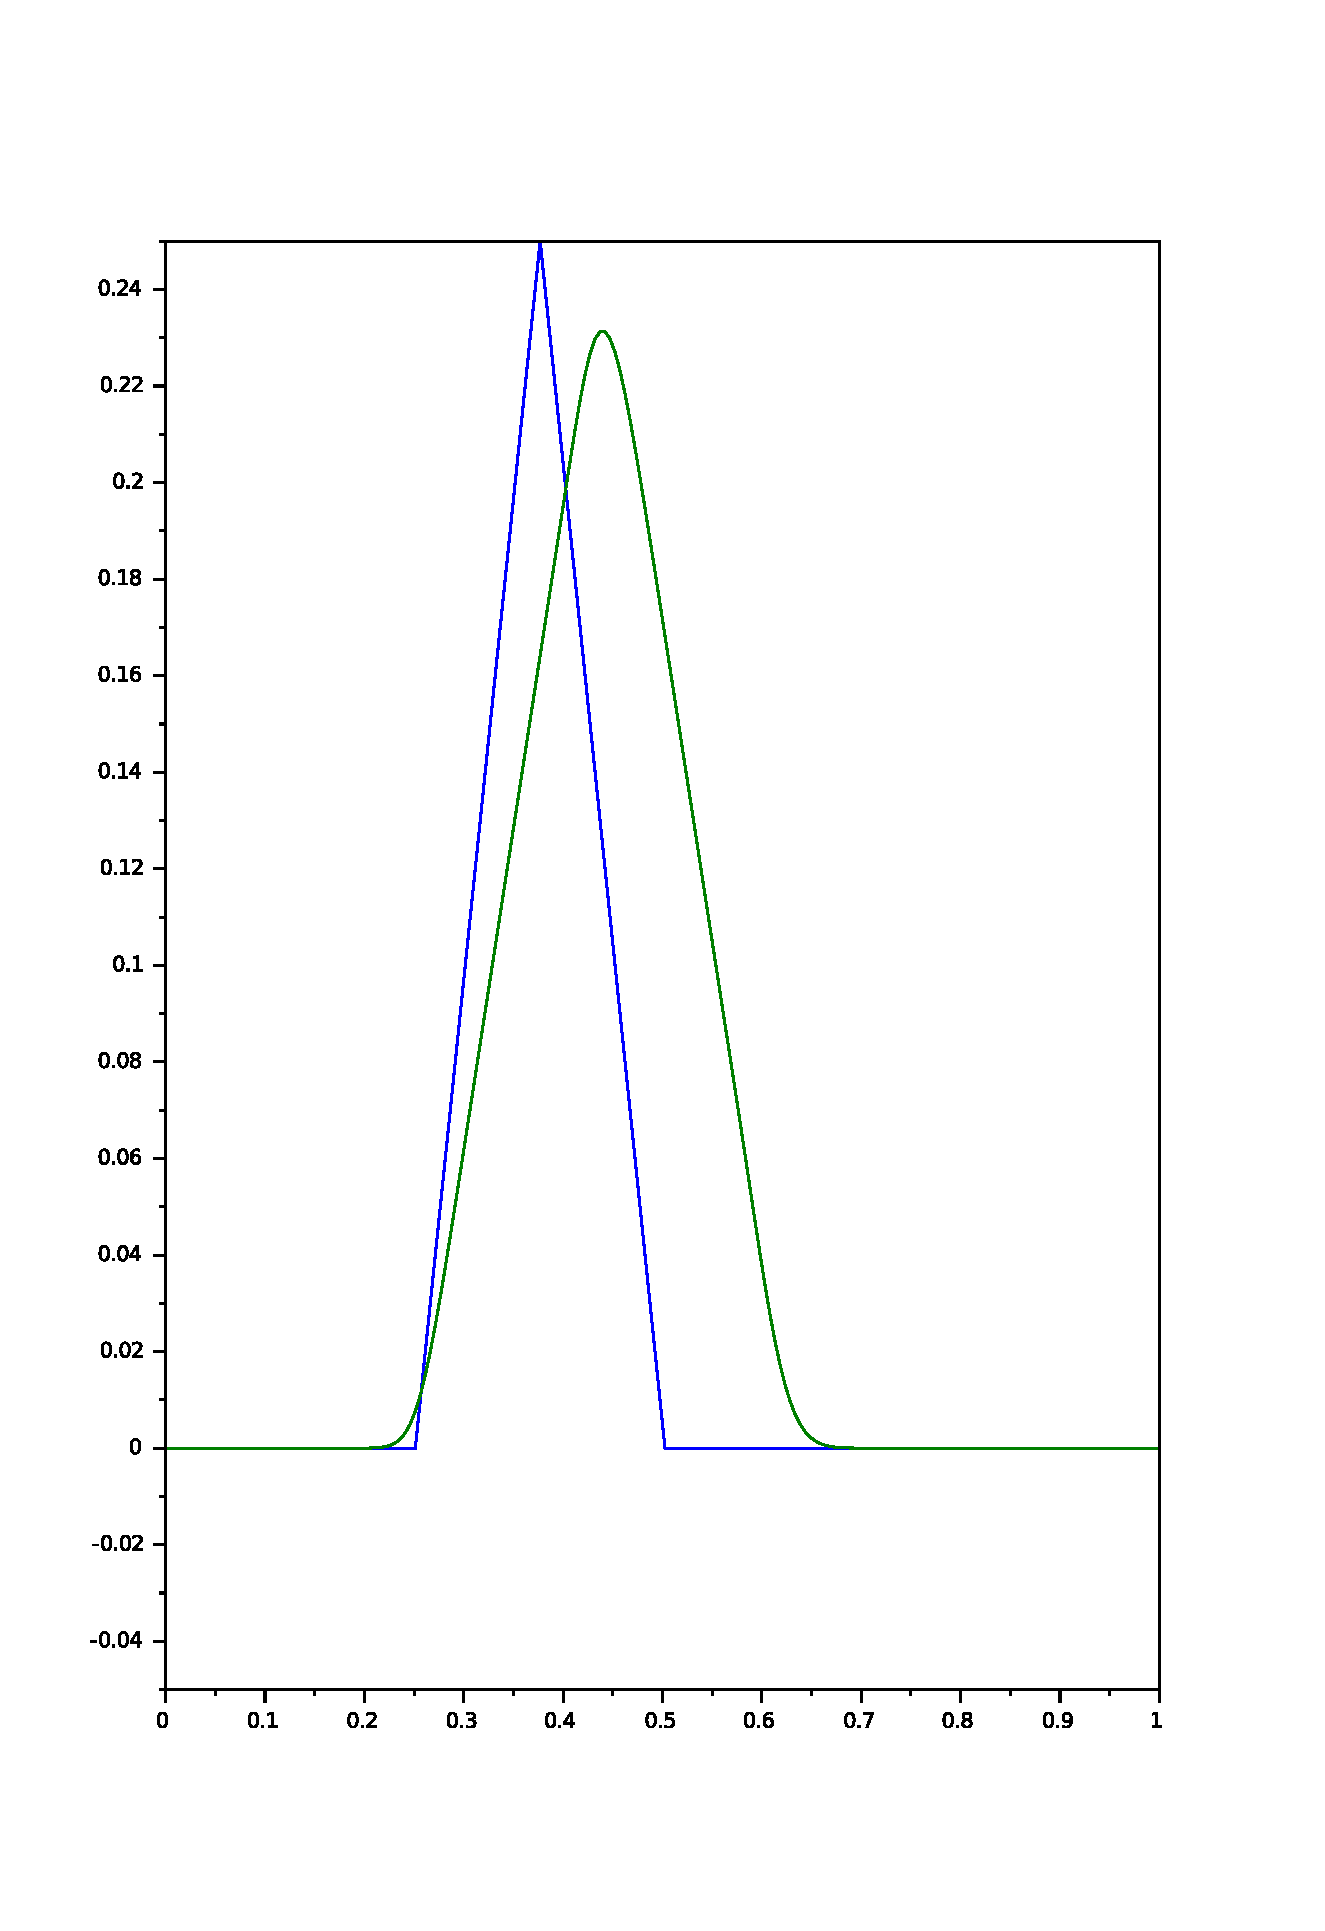
\includegraphics[width=\textwidth]{conv_kappa_0,0001.pdf}
		\caption{$\kappa=0.0001$}
	\end{subfigure}
	\caption{Diffusion pour differents $\kappa$}\label{fig:diff1D}
\end{figure}

On voit dans la figure~\ref{fig:diff1D} qu'il y a une plus grande diffusion plus $\kappa$ est grand. Cela est coherent etant donne que $\kappa$ est le coefficient qui quantifie la diffusion. Le schema semble bien donner la reponse attendue.

\paragraph{Question 5}

En resolvant les equations de diffusion sur les lignes puis les colonnes, grace a un solveur pour les matrices sparses on obtient des courbes montrant bien la diffusion periodique du systeme, comme le montre la figure~\ref{fig:diff2D}.

\begin{figure}
	\begin{subfigure}[b]{0.5\textwidth}
		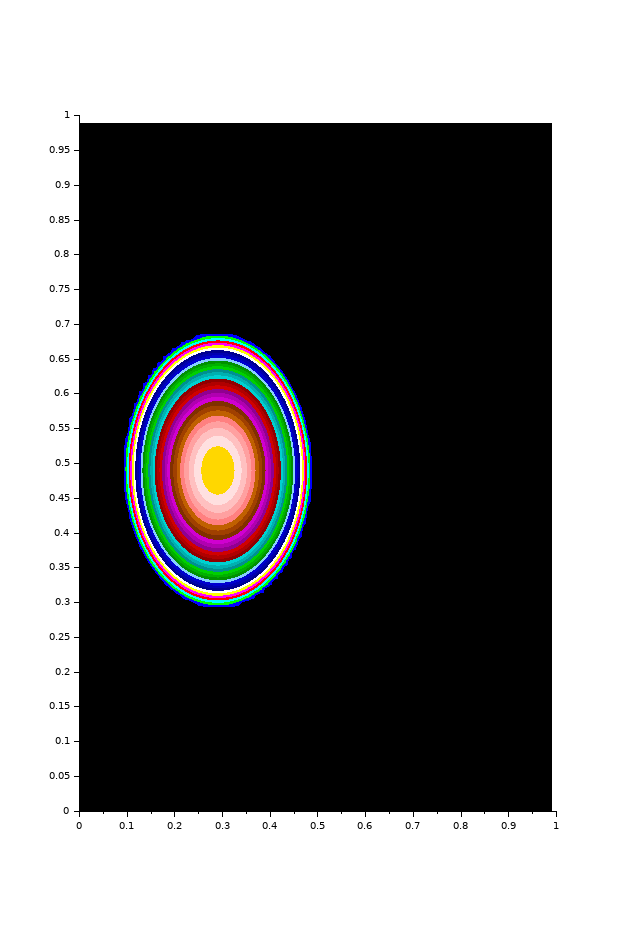
\includegraphics[width=\textwidth]{conv-2D_kappa_0,01_i.png}
		\caption{$t=0$}
	\end{subfigure}
	\begin{subfigure}[b]{0.5\textwidth}
		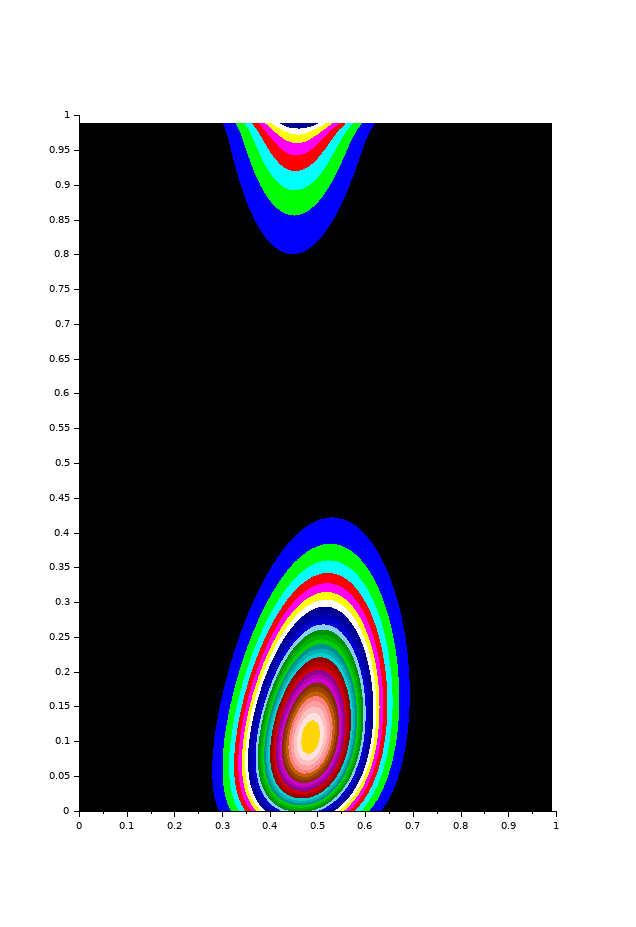
\includegraphics[width=\textwidth]{conv-2D_kappa_0,01_f.png}
		\caption{$t=t_f$}
	\end{subfigure}
	\caption{Diffusion en 2D pour $\kappa=0.01$}\label{fig:diff2D}
\end{figure}



\section{Resolution du problème de Poisson}

\paragraph{Question 6}
En appliquant l'equation (9) aux séries partielles, on a:
\begin{equation}
	\pd{S_{nm}(\psi)}{x^2}(x,y)
    + 
	\pd{S_{nm}(\psi)}{y^2}(x,y)
	= S_{nm}(f)(x,y)
    \label{eq:poisson}
\end{equation}
Et on obtient:
\begin{equation*}
    \sum_{p=-n}^{n} \sum_{q=-m}^{m} (\kxq^2 + \kyp^2) \hat{\psi}_{pq} e^{+\kyp y} e^{+\kxq x}
	=
		\sum_{p=-n}^{n} \sum_{q=-m}^{m}\hat{f}_{pq} e^{+\kyp y} e^{+\kxq x}
\end{equation*}
Comme la famille des \(((x, y)\mapsto e^{+\kyp y} e^{+\kxq x})_{(p,q)\in\mathbb N^2}\)
est libre, on obtient: pour tout \((p,q)\in\mathbb N^2\), \((\kxq^2 + \kyp^2) \hat{\psi}_{pq} = \hat{f}_{pq}\)
\\
Donc, pour \((p,q)\neq(0,0)\) on trouve \(\hat{\psi}_{pq} = \frac{\hat{f}_{pq}}{\kxq^2 + \kyp^2}\)

\paragraph{question 9}
Pour \(\alpha = \frac{1}{8\pi^2}\), on trouve bien :
\begin{align*}
	\Delta \hat{\psi}_{\alpha}(x,y) & = 2\times4\pi^2\alpha\sin(2\pi x)\sin(2\pi y)\\
	& = \sin(2\pi x)\sin(2\pi y)
\end{align*}

\end{document}
